%% Conclusion
%%=========================================

\chapter{Conclusion}
\label{ch:conclusion}
In this chapter we will summarize, and investigate, the results gathered throughout this thesis. We will state our final conclusion and look at potential future work.

%%=========================================

\section{Foobar}
In this section we reflect on our results in context of our research questions. Answering our research goal is done in the final conclusion.



\section{Discussion}
The results gathered from all the experiments ran as a part of this thesis indicates that both the encoder-decoder model were able to learn and generalize beyond the training sets.

\subsection{Encoding}
\red{Foobar}

\subsection{Decoding}
\red{Foobar}

\subsection{Use of Attention}
The experiments carried out in this thesis showed that both the models based on the encoder-decoder were powerful, but the model that utilized the attention mechanism was significantly better on the most complex experiment. Figure \ref{fig:attention_heatmap} shows the attention heatmap, in other words, the areas in which the attention mechanism focused while classifying each individual label. In this example the model correctly classifies the word ``IMAGINED" without any errors. 

The heatmap shows how the attention mechanism scanned both the related input, as well as input ahead of time, making use of the additional data to do the classifications. Comparing the heatmap in Figure \ref{fig:attention_heatmap} with the actual text and signature in Figure  \ref{fig:imagine_highlighted}\footnote{In this illustration the white pixels are highlighted in green, and black pixels are highlighted in red}, we can see that the heatmap focus almost matches the related input areas for each label. This additional information gives the {\tt EncDecAtt} a significant advantage over the {\tt EncDecReg} model, which can only rely on the information in the context vector. We see that this benefit pays off in the consistently better results the {\tt EncDegAtt} model has compared to the {\tt EncDecReg}.

\begin{figure}[h]
    \centering
    \includegraphics[width=1\textwidth]{fig/conclusion/attention_crop.png}
    \caption{Attention heatmap}
    \label{fig:attention_heatmap}
\end{figure}

\begin{figure}[h]
    \centering
    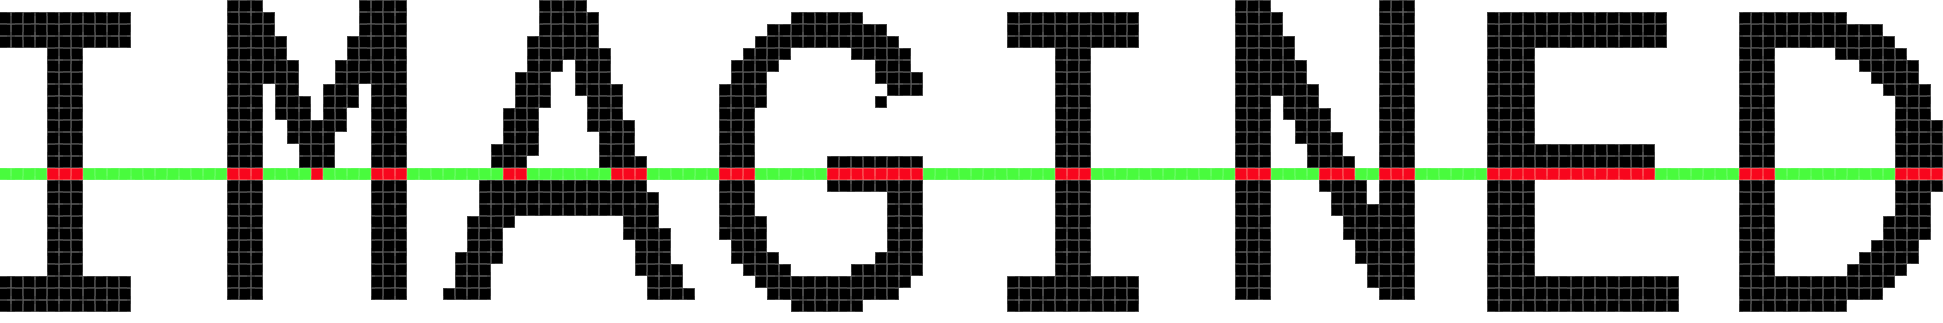
\includegraphics[width=1\textwidth]{fig/conclusion/imagined_grid_exported.png}
    \caption{The word ``IMAGINED" with the signature highlighted in red and green}
    \label{fig:imagine_highlighted}
\end{figure}

%%=========================================

\section{Conclusion}
As a result of research, we have developed two models based on the encoder-decoder framework that gave satisfying results on the experiments we carried out. Specifically, the {\tt EncoDecAtt} model had great results, even on the most complex experiments we carried out.

%%=========================================

\section{Future Work}
This thesis has looked closer at the possibilities the encoder-decoder opens up. We concluded that the framework worked 